\section{Алгоритм Бойера-Мура. Эвристики стоп-символа и хорошего суффикса.}

\textbf{Цель:} найти все вхождения шаблона в строку, используя при этом как можно меньше дополнительной памяти (в отличие от алгоритмов Кнута --- Морриса -- Пратта и Ахо --- Корасик)

\textbf{Идея:} возьмём базовый алгоритм для поиска за $O(nk)$
\begin{itemize}
	\item Проходимся по всем \textsf{str1} от $i$-го до $i+\text{len(str2)}-1$,
	\item Посимвольно сравниваем,
\end{itemize}
и попробуем его модернизировать

\textbf{Сам алгоритм}:
Будем сравнивать все символы в строке с символами подстроки \textbf{справа налево}. 
Если все символы шаблона совпали с наложенными символами строки, значит, подстрока найдена, и поиск окончен. 
В случае несовпадения какого-либо символа (или полного совпадения всего шаблона) он использует две предварительно вычисляемых эвристических функций, чтобы сдвинуть позицию для начала сравнения вправо.

Будем применять \textbf{две эвристики}:
\begin{itemize}
	\item Эвристика хорошего суффикса.
	\item Эвристика стоп-символа.
\end{itemize}

\subsection{Эвристика хорошего суффикса}

Если при сравнении текста и шаблона совпало один или больше символов, шаблон сдвигается в зависимости от того, какой суффикс совпал.

Если встретились оо
\begin{figure}[h!]
	\centering
	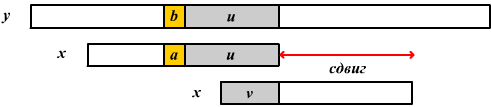
\includegraphics[width=0.7\linewidth]{img/10_1.png}
	\captionsetup{labelformat=empty}
	\caption{\textbf{Сдвиг хорошего суффикса}, вся подстрока u полностью встречается справа от символа c, отличного от символа a}
\end{figure}
kk
\begin{figure}[h!]
	\centering
	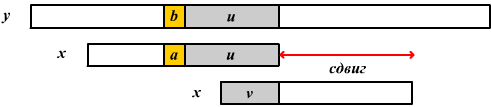
\includegraphics[width=0.7\linewidth]{img/10_2.png}
	\captionsetup{labelformat=empty}
	\caption{\textbf{Сдвиг хорошего суффикса}, только суффикс подстроки u повторно встречается в x.}
\end{figure}


\subsection{Эвристика стоп-символа}

На этапе инициализации составляется таблица плохих символов, в которой у каждого символа из алфавита отмечается последняя позиция его вхождения в шаблон.


\begin{figure}[h!]
	\centering
	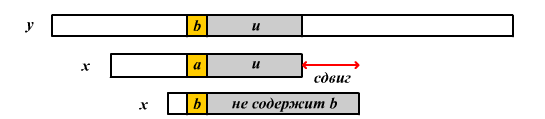
\includegraphics[width=0.7\linewidth]{img/10_3.png}
	\captionsetup{labelformat=empty}
	\caption{\textbf{Сдвиг плохого символа}, символ a входит в x.}
\end{figure}

\begin{figure}[h!]
	\centering
	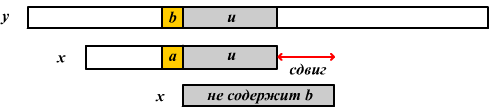
\includegraphics[width=0.7\linewidth]{img/10_4.png}
	\captionsetup{labelformat=empty}
	\caption{\textbf{Сдвиг плохого символа}, символ b не входит в x.}
\end{figure}


\subsection*{Доказательство корректности}

Для доказательства корректности алгоритма достаточно показать, что если та или иная эвристика предлагает сдвиг более чем на одну позицию вправо, на пропущенных позициях шаблон не найдётся.

Итак, пусть совпал суффикс $S$, строка-шаблон равна $PbS$, стоп-символ — $a$ (в дальнейшем малые буквы — символы, большие — строки).

\begin{figure}[h!]
	\centering
	
\includegraphics[width=0.7\linewidth]{img/10_5.png}
	\captionsetup{labelformat=empty}
	\caption{\textbf{}}
\end{figure}

\textbf{Эвристика стоп-символа.} 
Работает, когда в строке $V$ символ $а$ отсутствует. Если $P=WaV$ и в строке $V$ нет символа а, то эвристика стоп-символа предлагает сдвиг на $|V|+1$ позицию.

\begin{figure}[h!]
	\centering
	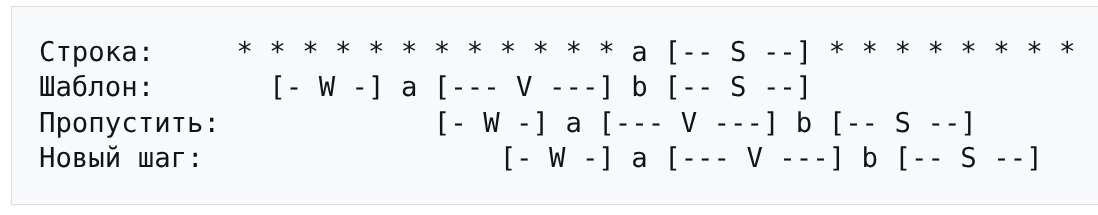
\includegraphics[width=0.8\linewidth]{img/10_6.png}
	\captionsetup{labelformat=empty}
	\caption{\textbf{}}
\end{figure}

Действительно, если в строке $V$ нет буквы a, нечего пробовать пропущенные $|V|$ позиций.
Если же в шаблоне нет символа а, то эвристика стоп-символа предлагает сдвиг на $|P|+1$ позицию — и также нет смысла пробовать пропущенные $|P|$.

\textbf{Эвристика совпавшего суффикса. }
Сама неформальная фраза — <<наименьшая величина, на которую нужно сдвинуть вправо шаблон, чтобы он снова совпал с $S$, но символ перед данным совпадением с $S$ (если такой символ существует) отличался бы от $b$>> — говорит, что меньшие сдвиги бесполезны.

\begin{figure}[h!]
	\centering
	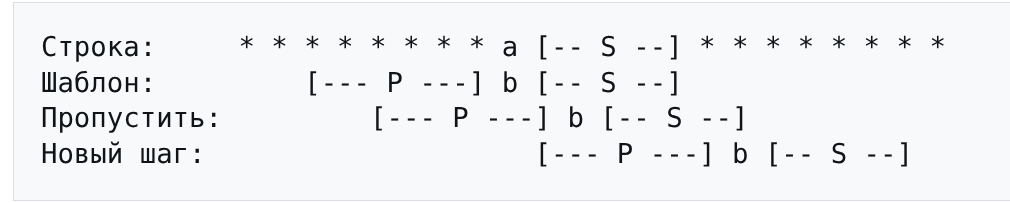
\includegraphics[width=0.8\linewidth]{img/10_7.png}
	\captionsetup{labelformat=empty}
	\caption{\textbf{}}
\end{figure}

